% ============================================================================
% Harvesting Idle CPU Cycles for LLM Inference:
% A Dual-Process Architecture for CPU-GPU Heterogeneous Serving
%
% IEEE Conference Format — Draft v4 — 2026-02-27
% ============================================================================

\documentclass[10pt,conference]{IEEEtran}

% --- Packages ---
\usepackage{amsmath,amssymb,amsfonts,amsthm}
\usepackage{algorithmic}
\usepackage[ruled,linesnumbered,vlined]{algorithm2e}
\usepackage{graphicx}
\usepackage{textcomp}
\usepackage{booktabs}
\usepackage{hyperref}
\usepackage{xcolor}
\usepackage{cite}
\usepackage{listings}
\usepackage{multirow}
\usepackage{balance}
\usepackage{pifont}
\usepackage{tikz}
\usepackage{pgfplots}
\pgfplotsset{compat=1.18}
\usetikzlibrary{shapes.geometric, arrows.meta, positioning, fit, backgrounds, calc, decorations.pathreplacing}

% --- Theorem environments ---
\newtheorem{theorem}{Theorem}
\newtheorem{corollary}[theorem]{Corollary}
\newtheorem{definition}[theorem]{Definition}
\newtheorem{property}{Property}

% --- Listings ---
\lstset{basicstyle=\ttfamily\footnotesize,breaklines=true,frame=none}

% ============================================================================
\title{The Forgotten Muscle:\\
Harvesting Idle CPU Compute for Additive-Throughput LLM Serving}

\author{
  \IEEEauthorblockN{Kyunam Cho\textsuperscript{1,2,3}}
  \IEEEauthorblockA{%
    \textsuperscript{1}Dept.\ of Computer Science and Engineering\\
    Korea University, Seoul, Republic of Korea\\
    \textsuperscript{2}LG Uplus Corp., Seoul, Republic of Korea\\
    \textsuperscript{3}School of Business, Ewha Womans University\\
    Seoul, Republic of Korea\\
    mystous@korea.ac.kr}
  \and
  \IEEEauthorblockN{Heonchang Yu\thanks{Corresponding author.}}
  \IEEEauthorblockA{%
    Dept.\ of Computer Science and Engineering\\
    Korea University, Seoul, Republic of Korea\\
    yuhc@korea.ac.kr}
}

% ============================================================================
\begin{document}
\maketitle

% --- Abstract ---
\begin{abstract}
The explosive growth of large language model (LLM) deployment has driven an unprecedented expansion of GPU infrastructure, with thousands of high-end GPU servers operating simultaneously to meet demand---incurring enormous capital and operational costs.
Within these servers, powerful multi-core CPUs are paired with GPU accelerators, yet the CPU remains almost entirely idle during inference---consuming power while producing no useful work.
Server-class CPUs have evolved dramatically alongside GPUs, now fielding hundreds of cores per socket and memory bandwidths approaching terabytes per second.
Yet during inference, the CPU is confined to auxiliary tasks---tokenization, request scheduling, and orchestrating the inference pipeline---never leveraging its substantial compute capability for the inference workload itself, leaving utilization below 5\%.
This idle power draw represents a significant energy inefficiency in an era where data centers already consume 4.4\% of U.S.\ electricity.
We present a dual-process parallel-batch architecture that engages both the CPU and GPU in inference computation, harvesting idle CPU cycles for productive LLM serving.
This approach is particularly effective during the memory-bandwidth-bound decode phase, where the CPU's bandwidth-to-compute ratio allows meaningful contribution.
Rather than sharing a single process between CPU and GPU, our approach runs each device as a fully independent inference engine in its own OS process, eliminating the interpreter lock contention, NUMA memory access penalties, and scheduling interference that would otherwise degrade GPU performance.
This process-level isolation eliminates software-level cross-device interference, yielding an additive throughput model: $T_\text{hybrid} = T_\text{GPU} + \alpha \cdot T_\text{CPU}$, subject to minimal hardware-level resource contention.
The two compute resources share inference workloads through capacity-aware distribution, exposed via a single API endpoint.
To ensure optimal CPU compute performance, the system automatically discovers hardware topology at startup to configure NUMA bindings, thread placement, and memory allocation without operator intervention.
The additional CPU compute throughput requires no new hardware procurement---only the marginal energy to move the CPU from idle to active---improving the server's overall performance-per-watt.
\end{abstract}

\begin{IEEEkeywords}
LLM inference, CPU-GPU heterogeneous computing, energy-proportional computing, process-level parallelism, resource harvesting
\end{IEEEkeywords}

% ============================================================================
\section{Introduction}
\label{sec:intro}

% --- Para 1: The paradox of idle power ---
The explosive growth of large language model (LLM) deployment has driven an unprecedented build-out of GPU infrastructure.
Thousands of high-end servers now operate around the clock to meet demand, each costing hundreds of thousands of dollars and drawing kilowatts of power.
Yet hidden inside every one of these GPU servers is a resource that nobody planned to leave idle: the host CPU.
Server-class CPUs have not stood still while GPUs advanced.
Intel's Xeon line tells a striking story of its own---Sapphire Rapids (2023) introduced 56~cores per socket with DDR5-4800 at 307\,GB/s and Advanced Matrix Extensions (AMX) for native BF16/INT8 acceleration; Emerald Rapids (2023) grew to 64~cores; Granite Rapids (2024) doubled again to 128~P-cores with 12-channel DDR5-6400 delivering 845\,GB/s per socket~\cite{na2024cpullm, intel2022amx}.
In just two generations, core count increased 2.3$\times$ and memory bandwidth 2.75$\times$---growth that, while not matching raw GPU compute scaling, has quietly made these CPUs formidable computing platforms in their own right.
In this work we target the widely deployed Sapphire Rapids platform (307\,GB/s); we note that the same architecture applied to Granite Rapids would yield proportionally larger CPU contributions.
These processors were engineered for heavy computation: dense linear algebra, cryptography, database analytics.
Yet when they are installed in a GPU inference server, all of that capability goes unused.
The CPU is confined to auxiliary bookkeeping---tokenization, request scheduling, orchestrating the inference pipeline---while the GPU alone performs every floating-point operation of the model~\cite{he2024xfastertransformer}.
The result is a striking paradox: 128~cores, terabytes of memory, and 845\,GB/s of bandwidth per socket sit idle at below 5\% utilization, a computational engine with no work to do.

% --- Para 2: The price of waste ---
This is not merely an aesthetic inefficiency; it has measurable costs at every scale.
At the level of a single server, an idle dual-socket Xeon still draws approximately 175\,W---a quarter of its thermal design power---consuming electricity solely to maintain readiness for work that never arrives~\cite{specpower2024}.
Zoom out to a 100-node GPU cluster running year-round, and that idle CPU power alone totals over 153\,MWh of wasted electricity (175\,W $\times$ 100 $\times$ 8{,}760\,h)---enough to power roughly 14 U.S.\ households for a year.
Zoom out further to the national scale: U.S.\ data centers consumed 176\,TWh in 2023, 4.4\% of the country's total electricity, and that figure is projected to double by 2028~\cite{lbnl2024datacenter}.
Every watt that a server draws without producing useful work pushes the industry further from Barroso and H\"{o}lzle's vision of \emph{energy-proportional computing}, where power consumption scales with actual utilization~\cite{barroso2007energy}.
The capital dimension compounds the problem: the CPU and memory subsystem in each server represents \$30--50K in hardware investment that yields near-zero return during inference---millions of dollars in stranded assets across a single cluster.
These observations lead to a natural research question: \emph{Can we harvest idle CPU cycles for productive LLM inference without degrading GPU throughput---thereby converting wasted power into useful work?}

% --- Para 3: Why previous approaches fell short ---
The idea of engaging the CPU in inference is not new, but prior efforts have consistently fallen short (Section~\ref{sec:related-hetero}).
Existing heterogeneous systems---spanning neuron-level partitioning~\cite{song2024powerinfer}, attention offloading~\cite{neo2025}, and speculative-decoding drafting~\cite{dovetail2024, apex2025}---all share a common architectural constraint: CPU and GPU execution coexist inside the same OS process.
This triggers a cascade of entangled problems: Python's Global Interpreter Lock (GIL) serializes control flow, NUMA architectures impose steep penalties when threads inadvertently access remote memory, and any CPU-side computation risks interfering with GPU kernel launches and memory transfers.
The cumulative effect is a lose-lose dilemma: single-process hybrid designs either sacrifice GPU throughput to accommodate the CPU, or constrain CPU utilization to avoid disturbing the GPU.

% --- Para 4: Our insight and approach ---
Our \textbf{key insight} is that these barriers are not inherent to heterogeneous inference; they are artifacts of sharing a single process.
By running each device as a \emph{fully independent inference engine in its own OS process}---with its own interpreter lock, memory space, and NUMA binding---we eliminate software-level sources of cross-device interference at once.
The result is a clean, additive throughput model:
\[
T_\text{hybrid} = T_\text{GPU} + \alpha \cdot T_\text{CPU}, \quad \alpha \in [0, 1]
\]
where $\alpha$ captures router efficiency (formalized in Section~\ref{sec:throughput-model}) and GPU performance remains completely undisturbed.
This is \emph{not} simply running two separate serving instances: the GPU and CPU engines share a single API endpoint, a unified request router that directs traffic based on real-time CPU capacity, and an automatic hardware-discovery pipeline that configures NUMA bindings and thread placement at startup without operator intervention.
Rather than asking ``how much CPU work can we tolerate before the GPU slows down,'' we reframe the question as ``how much \emph{additional} throughput can the CPU deliver using resources that are already powered on?''
Because the CPU engine targets the memory-bandwidth-bound decode phase---where the speed gap to the GPU is narrow enough for meaningful contribution---even a modest CPU throughput adds directly to the server's total output.
For models that fit in the server's existing DRAM (which already provisions terabytes for GPU host memory), this additional throughput comes with no new hardware procurement; the only incremental cost is the marginal power to move the CPU from idle to active.

% --- Para 5: Contributions ---
Based on this insight, we present a system that engages \textbf{both the CPU and GPU in inference computation} and make the following contributions:
\begin{enumerate}
\item A \textbf{dual-process parallel-batch architecture} that runs GPU and CPU as independent inference engines with an additive throughput model and analysis of GPU latency preservation (Section~\ref{sec:design}).
The primary contribution is the \emph{systems integration}---demonstrating that process-level isolation, combined with capacity-aware routing and automatic hardware discovery, makes heterogeneous CPU-GPU inference practical within a production serving framework.
\item A \textbf{self-regulating CapacityAwareRouter} with three routing strategies---capacity-based, length-aware, and throughput-adaptive---that maximizes CPU utilization without manual tuning (Section~\ref{sec:router}).
\item A \textbf{zero-configuration hardware discovery pipeline} that automatically detects NUMA topology, ISA capabilities, and optimal thread bindings at startup (Section~\ref{sec:autoconfig}).
\item An analysis demonstrating that \textbf{idle CPU power can be converted to productive inference}, improving server-level performance-per-watt with no additional hardware procurement---only the marginal energy to move the CPU from idle to active (Section~\ref{sec:discussion}).
\end{enumerate}

% ============================================================================
\section{Background and Motivation}
\label{sec:background}

\subsection{LLM Inference Characteristics}
\label{sec:bg-llm}

LLM inference proceeds in two distinct phases with contrasting computational profiles~\cite{agrawal2023sarathi, agrawal2024sarathiserve}.
The \emph{prefill} phase processes all input tokens in parallel through the model, performing dense matrix multiplications that are \emph{compute-bound}.
The \emph{decode} phase generates output tokens one at a time, where each step requires loading the full model weights and KV cache from memory but performs minimal computation---making it \emph{memory-bandwidth-bound}.

This memory-bound nature of decoding has a crucial implication: \emph{any device with sufficient memory bandwidth can contribute to decode throughput}, regardless of its raw compute capability.
For a model with $P$ parameters at $b$ bytes per parameter, the theoretical maximum decode throughput is:
\begin{equation}
\label{eq:roofline}
T_\text{decode} = \frac{B_\text{mem}}{P \times b} \quad \text{tokens/s}
\end{equation}
where $B_\text{mem}$ is the device's memory bandwidth.
For a Xeon 8480+ with 8-channel DDR5-4800, each socket provides approximately 307\,GB/s of memory bandwidth. Since the CPU engine binds to a single NUMA node (one socket), 307\,GB/s is the effective bandwidth available, yielding a theoretical decode rate of 4.4\,tokens/s for a 70B-parameter model in Q8\_0 quantization (70\,GB effective weight size).
While modest compared to H100 GPU bandwidth (3.35\,TB/s), this represents \emph{free} additional throughput from otherwise idle hardware.
We formalize this bandwidth-determined throughput ratio and its implications for multi-GPU tensor parallelism in Section~\ref{sec:throughput-model}.

\begin{figure}[t]
\centering
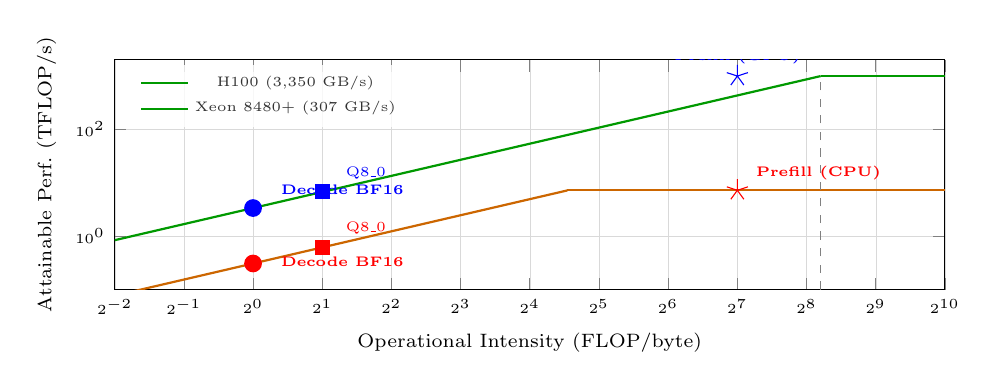
\begin{tikzpicture}
\begin{axis}[
    width=\columnwidth,
    height=4.5cm,
    xmode=log,
    ymode=log,
    log basis x=2,
    log basis y=10,
    xlabel={Operational Intensity (FLOP/byte)},
    ylabel={Attainable Perf.\ (TFLOP/s)},
    xmin=0.25, xmax=1024,
    ymin=0.1, ymax=2000,
    grid=both,
    grid style={line width=0.1pt, draw=gray!30},
    legend style={at={(0.02,0.98)}, anchor=north west, font=\tiny, draw=none, fill=white, fill opacity=0.8},
    tick label style={font=\tiny},
    label style={font=\scriptsize},
  ]
  \addplot[thick, color=green!60!black, domain=0.25:295] {3.35 * x};
  \addplot[thick, color=green!60!black, domain=295:1024] {989};
  \addlegendentry{H100 (3,350 GB/s)}
  \addplot[thick, color=orange!80!black, domain=0.25:23.3] {0.307 * x};
  \addplot[thick, color=orange!80!black, domain=23.3:1024] {7.2};
  \addlegendentry{Xeon 8480+ (307 GB/s)}
  \addplot[only marks, mark=*, mark size=3pt, color=blue] coordinates {(1, 3.35)};
  \node[anchor=south west, font=\tiny\bfseries, color=blue] at (axis cs:1.2, 4.0) {Decode BF16};
  \addplot[only marks, mark=*, mark size=3pt, color=red] coordinates {(1, 0.307)};
  \node[anchor=south west, font=\tiny\bfseries, color=red] at (axis cs:1.2, 0.18) {Decode BF16};
  \addplot[only marks, mark=square*, mark size=2.5pt, color=blue] coordinates {(2, 6.7)};
  \node[anchor=south west, font=\tiny, color=blue] at (axis cs:2.3, 7.5) {Q8\_0};
  \addplot[only marks, mark=square*, mark size=2.5pt, color=red] coordinates {(2, 0.614)};
  \node[anchor=south west, font=\tiny, color=red] at (axis cs:2.3, 0.7) {Q8\_0};
  \addplot[only marks, mark=star, mark size=4pt, color=blue] coordinates {(128, 989)};
  \node[anchor=south, font=\tiny\bfseries, color=blue] at (axis cs:128, 1100) {Prefill (GPU)};
  \addplot[only marks, mark=star, mark size=4pt, color=red] coordinates {(128, 7.2)};
  \node[anchor=south west, font=\tiny\bfseries, color=red] at (axis cs:140, 7.5) {Prefill (CPU)};
  \draw[dashed, thin, gray] (axis cs:295,0.1) -- (axis cs:295,989);
\end{axis}
\end{tikzpicture}
\caption{Roofline model for H100 GPU and Xeon 8480+ CPU. The decode phase (OI $= 1$ for BF16, $= 2$ for Q8\_0) falls deep in the memory-bandwidth-bound region for both devices, while prefill operates near the compute ceiling. The CPU's decode throughput is determined entirely by its memory bandwidth.}
\label{fig:roofline}
\end{figure}

Figure~\ref{fig:roofline} visualizes this relationship using the roofline model: both prefill and decode phases are plotted against each device's performance ceiling, confirming that decode throughput is bottlenecked by memory bandwidth rather than compute.

\subsection{vLLM: A Multi-Process Serving Architecture}
\label{sec:bg-vllm}

Our work builds on vLLM~\cite{kwon2023vllm}, a widely adopted open-source LLM serving engine.
Two architectural properties of vLLM make it a natural foundation for CPU-GPU hybrid inference.

First, vLLM's \emph{EngineCore} abstraction cleanly separates inference orchestration from device-specific execution.
The EngineCore manages the scheduling loop---continuous batching~\cite{yu2022orca}, KV cache allocation via PagedAttention, and request lifecycle management---while delegating tensor computation to a pluggable executor layer.
This separation means the same EngineCore can drive either a GPU executor (MultiprocExecutor with tensor parallelism across multiple GPUs) or a CPU executor (UniProcExecutor with a single CPUWorker), without any modification to the core scheduling logic.

Second, vLLM already employs \emph{process-level isolation} for its GPU engine: the EngineCoreProc wrapper spawns the EngineCore in a dedicated child process, communicating with the frontend via ZMQ IPC sockets~\cite{hintjens2013zeromq}.
This existing multi-process infrastructure---process spawning, IPC message framing, and asynchronous result collection---provides the scaffolding for our dual-process design.
Rather than building a hybrid serving system from scratch, we launch a second EngineCoreProc for the CPU engine alongside the existing GPU process, reusing the same IPC protocol and adding only a routing layer (Section~\ref{sec:design}).
The GPU code path remains entirely unmodified.

\subsection{The Idle CPU Problem: Power and Cost}
\label{sec:bg-idle}

Table~\ref{tab:idle-resources} quantifies the resource utilization and power characteristics of a representative GPU inference server during LLM serving.
The GPU subsystem operates at 60--90\% utilization, while CPU and memory resources---which together account for approximately 255\,W of idle power draw and \$30--50K of hardware cost---remain almost entirely unused.

\begin{table}[t]
\centering
\caption{Resource utilization and power in a DGX H100 server during LLM inference. CPU and memory resources consume power while producing no useful inference work.}
\label{tab:idle-resources}
\footnotesize
\begin{tabular}{@{}llrrr@{}}
\toprule
\textbf{Resource} & \textbf{Specification} & \textbf{Util.} & \textbf{Idle} & \textbf{Power} \\
\midrule
GPU Compute & 8$\times$ H100 SXM5 & 60--90\% & --- & 5,600\,W \\
GPU Memory & 640\,GB HBM3 & 70--95\% & --- & (incl.) \\
\midrule
CPU Compute & 2$\times$ Xeon 8480+ & $<$5\% & $>$106 cores & $\sim$175\,W \\
System Memory & 2\,TB DDR5-4800 & $<$10\% & $>$1.8\,TB & $\sim$80\,W \\
Mem.\ Bandwidth & 307\,GB/s (per-socket) & $<$3\% & 298\,GB/s & (incl.) \\
\bottomrule
\end{tabular}
\end{table}

Barroso and H\"{o}lzle's seminal work on energy-proportional computing~\cite{barroso2007energy} argued that servers should consume power proportional to their utilization.
Nearly two decades later, the SPECpower benchmark shows that idle servers still draw approximately 25\% of their peak power~\cite{specpower2024}.
GPU inference servers exemplify this anti-pattern at the subsystem level: the CPU subsystem draws 175\,W while performing effectively zero productive work.
Our approach directly addresses this energy inefficiency by converting idle CPU cycles into productive inference, moving the server closer to energy proportionality.

The economic argument is equally compelling.
In a 100-node cluster, the stranded CPU/memory investment exceeds \$3M, and the wasted idle power costs approximately \$18.4K annually (175\,W $\times$ 100 $\times$ 8{,}760\,h $\times$ \$0.12/kWh).
Even a modest 3\% throughput improvement from CPU utilization translates to the equivalent of three additional GPU servers (\$900K value)---achieved at zero additional hardware cost and minimal incremental power.

These observations motivate a natural research agenda: harvesting these idle resources for productive inference.
However, as we discuss in Section~\ref{sec:related}, existing heterogeneous inference approaches all operate within a single OS process, inheriting fundamental limitations that our dual-process design eliminates (Section~\ref{sec:design}).

% ============================================================================
\section{Related Work}
\label{sec:related}

\subsection{GPU-Centric LLM Serving}
The modern LLM serving stack has been shaped by a series of GPU-focused innovations.
Orca~\cite{yu2022orca} introduced continuous (iteration-level) batching, eliminating padding waste and enabling concurrent prefill and decode.
vLLM~\cite{kwon2023vllm} added PagedAttention to virtualize KV cache memory, reducing fragmentation to near zero and increasing throughput 2--4$\times$.
SGLang~\cite{zheng2024sglang} optimized structured generation with RadixAttention for prefix caching, and Sarathi-Serve~\cite{agrawal2024sarathiserve} resolved the throughput-latency tradeoff through chunked prefills.
DeepSpeed-FastGen~\cite{holmes2024deepspeedfastgen} proposed Dynamic SplitFuse to decompose long prompts across multiple forward passes.
Megatron-LM~\cite{shoeybi2019megatron} established tensor and pipeline parallelism patterns that underpin multi-GPU serving today.
All of these systems treat the host CPU as a control-plane resource; our work is complementary, adding a CPU data-plane execution path while preserving all existing GPU optimizations.

\subsection{Intra-Request CPU-GPU Heterogeneous Inference}
\label{sec:related-hetero}
A growing body of work partitions \emph{individual requests} across CPU and GPU.
Table~\ref{tab:comparison} summarizes the key architectural differences.

\begin{table}[t]
\centering
\caption{Comparison of heterogeneous LLM inference approaches. Existing systems partition work \emph{within} a single request (intra-request), sharing a process and GIL. Our approach routes \emph{entire requests} to independent processes (inter-request).}
\label{tab:comparison}
\footnotesize
\begin{tabular}{@{}lcccc@{}}
\toprule
\textbf{System} & \textbf{Granularity} & \textbf{Process} & \textbf{GPU} & \textbf{Auto} \\
 & & \textbf{Isolation} & \textbf{Interf.} & \textbf{Config} \\
\midrule
PowerInfer~\cite{song2024powerinfer} & Neuron & \ding{55} & High & \ding{55} \\
KTransformers~\cite{chen2025ktransformers} & Expert & \ding{55} & Medium & \ding{55} \\
HeteGen~\cite{zhao2024hetegen} & Layer & \ding{55} & Medium & \ding{55} \\
NEO~\cite{neo2025} & Attention & \ding{55} & Low & \ding{55} \\
APEX~\cite{apex2025} & Batch & \ding{55} & Low & \ding{55} \\
Dovetail~\cite{dovetail2024} & Draft/Verify & \ding{55} & Medium & \ding{55} \\
FlexInfer~\cite{na2025flexinfer} & Phase & \ding{55} & Low & \ding{55} \\
Fiddler~\cite{kamahori2025fiddler} & Expert & \ding{55} & Medium & \ding{55} \\
\midrule
\textbf{This work} & \textbf{Request} & \ding{51} & \textbf{Zero} & \ding{51} \\
\bottomrule
\end{tabular}
\end{table}

PowerInfer~\cite{song2024powerinfer} exploits activation sparsity to route hot neurons to the GPU and cold neurons to the CPU---effective on consumer hardware but tightly coupling the two devices within a single forward pass.
PowerInfer-2~\cite{xue2024powerinfer2} extends this to mobile XPUs (big.LITTLE CPU, GPU, NPU) via neuron-cluster scheduling.
KTransformers~\cite{chen2025ktransformers} offloads MoE experts to CPU, and HeteGen~\cite{zhao2024hetegen} pipelines layer-level computation across devices asynchronously, achieving 317\% speedup over CPU-only baselines.
NEO~\cite{neo2025} moves attention to the CPU while the GPU handles feed-forward layers, and APEX~\cite{apex2025} overlaps CPU and GPU execution at the batch level.
Dovetail~\cite{dovetail2024} uses the CPU as a speculative-decoding draft generator.
Despite varying granularities, all these systems operate within a single OS process, inheriting GIL contention, shared-memory NUMA penalties, and unavoidable GPU scheduling interference.
A direct comparison is instructive: PowerInfer achieves $11{\times}$ speedup over CPU-only but requires intrusive model-level modifications (neuron-level routing tables, activation predictors); HeteGen's asynchronous layer pipelining reports $3.17{\times}$ over CPU-only but still couples CPU and GPU within a shared process, limiting GPU throughput under high load.
Our approach departs from this paradigm entirely by routing \emph{whole requests}---not tensors or layers---to independent processes, eliminating cross-device interference by construction.
The trade-off is that we sacrifice within-request CPU-GPU cooperation (which could accelerate individual requests) in favor of system-level throughput isolation (which guarantees no GPU performance degradation).

\subsection{Memory and Expert Offloading}
A large body of work uses CPU memory and compute to extend GPU capacity, spanning weight offloading, MoE expert management, and phase-aware CPU execution.

\textbf{Weight offloading.}
FlexGen~\cite{sheng2023flexgen} formulates GPU/CPU/disk tensor placement as a linear program, enabling a single 16\,GB GPU to serve OPT-175B via aggressive offloading and 4-bit compression---at the cost of high latency per token.
DeepSpeed-Inference~\cite{aminabadi2022deepspeed} provides ZeRO-Inference for heterogeneous offloading of model weights to CPU DRAM and NVMe, targeting models too large for GPU memory.
LLM in a Flash~\cite{alizadeh2024flash} optimizes flash-to-DRAM transfers with windowing and row-column bundling to serve models that exceed available DRAM.

\textbf{MoE expert offloading.}
The sparse activation pattern of Mixture-of-Experts models makes CPU offloading particularly attractive, as only a fraction of experts are active per token.
Pre-gated MoE~\cite{hwang2024pregated} introduces a pre-gating function that predicts the next block's active experts during the current block's execution, overlapping CPU-to-GPU expert transfers with computation (ISCA~2024).
Fiddler~\cite{kamahori2025fiddler} generates hardware-aware execution strategies that orchestrate CPU and GPU for MoE inference, minimizing expert transfer overhead (ICLR~2025).
MoE-Lightning~\cite{cao2025moelightning} achieves high-throughput MoE serving on memory-constrained GPUs through a CGOPipe schedule that pipelines CPU, GPU, and I/O stages, reporting up to 10.3$\times$ throughput over baselines (ASPLOS~2025).

\textbf{Phase-aware CPU computation.}
FlexInfer~\cite{na2025flexinfer} goes beyond passive offloading by using a performance estimator to dynamically select optimal CPU-GPU execution policies for each inference phase (prefill vs.\ decode), achieving 75--76\% latency reduction over FlexGen (MLSys~2025).

All of these approaches use the CPU to \emph{supplement} a single GPU process---whether as passive storage, expert cache, or phase-specific accelerator.
Our system treats the CPU as a \emph{fully independent inference engine} in a separate OS process, running its own scheduling loop and serving entire requests in parallel with the GPU.

\subsection{Speculative Decoding}
Speculative decoding~\cite{leviathan2023speculative, chen2023speculative} accelerates autoregressive generation by having a small draft model propose multiple tokens that the target model verifies in a single forward pass, preserving output distribution exactly.
Medusa~\cite{cai2024medusa} eliminates the separate draft model entirely, attaching lightweight decoding heads to the target model for 2--3$\times$ speedup.
EAGLE~\cite{li2024eagle} achieves higher acceptance rates by operating at the feature level rather than the token level, reaching $\sim$3$\times$ acceleration.
While Dovetail~\cite{dovetail2024} combines speculative decoding with CPU-GPU heterogeneity, it couples the draft and verify stages within one process.
Our architecture is orthogonal to speculative decoding: the CPU engine could itself employ draft-and-verify internally while remaining fully isolated from the GPU engine.

\subsection{Disaggregated Serving}
DistServe~\cite{zhong2024distserve} and Splitwise~\cite{patel2024splitwise} (ISCA Best Paper Nominee) separate the compute-bound prefill and memory-bound decode phases onto different GPU pools, each optimized independently---Splitwise reports 1.4$\times$ throughput at 20\% lower cost.
Mooncake~\cite{qin2025mooncake} (FAST Best Paper) takes a KVCache-centric approach, using idle CPU/DRAM/SSD on GPU nodes as a distributed cache layer to reduce redundant prefill computation, achieving up to 525\% throughput gain.
Our dual-process architecture shares the disaggregation philosophy---separating concerns onto dedicated hardware---but applies it along the \emph{device} axis (CPU vs.\ GPU) rather than the \emph{phase} axis (prefill vs.\ decode), and the two approaches are composable.

\subsection{Energy-Efficient AI and Sustainable Computing}
Barroso and H\"{o}lzle~\cite{barroso2007energy} argued that servers should consume power proportional to their utilization; nearly two decades later, idle servers still draw $\sim$25\% of peak power~\cite{specpower2024}.
Strubell et al.~\cite{strubell2019energy} quantified the financial and environmental cost of training large NLP models, and Patterson et al.~\cite{patterson2021carbon} estimated that training GPT-3 emits $\sim$552 tonnes of CO$_2$.
Wu et al.~\cite{wu2022sustainable} broadened the lens to the full AI lifecycle, noting that inference accounts for 80--90\% of ML energy consumption in production and advocating hardware-software co-design for sustainability.
Our work directly addresses the inference-time energy gap: by converting idle CPU power into productive throughput, we move GPU servers closer to energy proportionality without additional hardware procurement.

% ============================================================================
\section{System Design}
\label{sec:design}

\subsection{Architecture Overview}

The system consists of three components: a routing layer (HybridAsyncMPClient), a GPU inference process, and a CPU inference process, connected via ZMQ IPC sockets.
The router dispatches entire requests to either engine via a ZMQ ROUTER socket with identity-based addressing; results are collected asynchronously through a shared ZMQ PULL socket.
Figure~\ref{fig:architecture} illustrates the overall architecture.

\begin{figure}[t]
\centering
\resizebox{\columnwidth}{!}{%
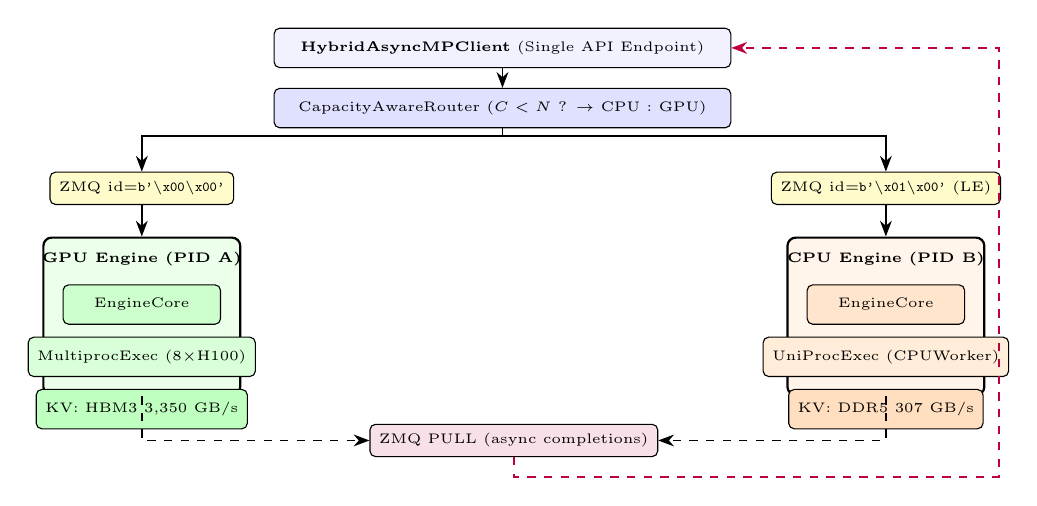
\begin{tikzpicture}[
    >=Stealth,
    node distance=0.4cm,
    box/.style={draw, rounded corners=2pt, minimum width=1.9cm, minimum height=0.5cm, align=center, font=\tiny},
    bigbox/.style={draw, rounded corners=3pt, thick, align=center, font=\tiny},
    sock/.style={draw, fill=yellow!20, rounded corners=2pt, minimum width=1.4cm, minimum height=0.35cm, align=center, font=\tiny},
    arrow/.style={->, semithick},
  ]
  % Client
  \node[box, fill=blue!5, minimum width=5.8cm] (client) {\textbf{HybridAsyncMPClient} (Single API Endpoint)};
  % Router
  \node[box, fill=blue!12, minimum width=5.8cm, below=0.25cm of client] (router) {CapacityAwareRouter ($C < N$ ? $\to$ CPU : GPU)};
  \draw[arrow] (client) -- (router);
  % ZMQ sockets
  \node[sock, below left=0.55cm and 0.5cm of router] (zmq_g) {ZMQ id=\texttt{b'\textbackslash{}x00\textbackslash{}x00'}};
  \node[sock, below right=0.55cm and 0.5cm of router] (zmq_c) {ZMQ id=\texttt{b'\textbackslash{}x01\textbackslash{}x00'} (LE)};
  \draw[arrow] (router.south) -- ++(0,-0.1) -| (zmq_g.north);
  \draw[arrow] (router.south) -- ++(0,-0.1) -| (zmq_c.north);
  % GPU Engine
  \node[bigbox, fill=green!8, below=0.4cm of zmq_g, minimum width=2.5cm, minimum height=2.0cm] (gpu) {};
  \node[font=\tiny\bfseries, anchor=north] at ([yshift=-0.08cm]gpu.north) {GPU Engine (PID A)};
  \node[box, fill=green!20, minimum width=2.0cm] at ([yshift=0.15cm]gpu.center) (gc) {EngineCore};
  \node[box, fill=green!15, minimum width=2.0cm, below=0.15cm of gc] (ge) {MultiprocExec (8$\times$H100)};
  \node[box, fill=green!25, minimum width=2.0cm, below=0.15cm of ge] (gk) {KV: HBM3 3,350 GB/s};
  \draw[arrow] (zmq_g) -- (gpu);
  % CPU Engine
  \node[bigbox, fill=orange!8, below=0.4cm of zmq_c, minimum width=2.5cm, minimum height=2.0cm] (cpu) {};
  \node[font=\tiny\bfseries, anchor=north] at ([yshift=-0.08cm]cpu.north) {CPU Engine (PID B)};
  \node[box, fill=orange!20, minimum width=2.0cm] at ([yshift=0.15cm]cpu.center) (cc) {EngineCore};
  \node[box, fill=orange!15, minimum width=2.0cm, below=0.15cm of cc] (ce) {UniProcExec (CPUWorker)};
  \node[box, fill=orange!25, minimum width=2.0cm, below=0.15cm of ce] (ck) {KV: DDR5 307 GB/s};
  \draw[arrow] (zmq_c) -- (cpu);
  % PULL socket
  \node[sock, fill=purple!12, below=0.35cm of $(gpu.south)!0.5!(cpu.south)$, minimum width=3.2cm] (pull) {ZMQ PULL (async completions)};
  \draw[arrow, dashed] (gpu.south) |- (pull.west);
  \draw[arrow, dashed] (cpu.south) |- (pull.east);
  \draw[arrow, dashed, purple] (pull.south) -- ++(0,-0.25) -| ([xshift=3.4cm]client.east) -- (client.east);
\end{tikzpicture}%
}
\caption{Dual-process hybrid architecture. The CapacityAwareRouter dispatches requests to either the GPU or CPU engine process via identity-based ZMQ sockets. Each engine runs in a separate OS process with independent scheduling loops, KV caches, and executors. Completions are collected asynchronously through a shared PULL socket.}
\label{fig:architecture}
\end{figure}

The design adheres to five principles:

\begin{enumerate}
\item \textbf{Process Isolation}: Separate PID, GIL, and address space per engine, ensuring zero mutual interference.
\item \textbf{Minimal Modification}: The GPU engine's EngineCore runs entirely unmodified; hybrid logic resides only in the routing layer.
\item \textbf{Capacity-Based Routing}: Requests are routed at the request level based on CPU slot availability, not token-level partitioning.
\item \textbf{Zero Configuration}: CPU parameters (threads, KV cache, batch size) are automatically derived from hardware topology.
\item \textbf{Energy Harvesting}: Idle CPU cycles are converted to productive inference, improving performance-per-watt without additional hardware.
\end{enumerate}

\textbf{Why separate processes?}
A natural alternative is running CPU and GPU inference within a single process, avoiding IPC overhead.
We chose process isolation for three reasons: (1)~Python's GIL creates contention between the GPU engine's scheduling loop and any CPU-bound computation in the same process---while PyTorch's C++ kernels release the GIL during execution, the Python-level scheduling, batching, and sampling code does not;
(2)~NUMA-aware memory allocation requires per-process binding (via \texttt{numactl} or \texttt{libnuma}), which cannot be applied to individual threads within a shared process;
(3)~independent processes provide natural fault isolation---a CPU engine crash does not affect the GPU process.
The ZMQ IPC overhead (${\sim}11$\,\textmu{}s per routing decision) is negligible relative to inference latency.

\subsection{Throughput Model}
\label{sec:throughput-model}

The architecture's value proposition rests on two claims: (1)~throughput is additive---the CPU contribution does not come at the expense of GPU performance, and (2)~the routing overhead is negligible.
We now model both claims and discuss the conditions under which they hold.
Because the GPU and CPU engines execute as independent OS processes with no shared mutable state (as established in the architecture overview above), their throughputs are expected to compose additively.

\begin{definition}[Hybrid Throughput]
\label{def:throughput}
Let $T_\text{GPU}$ and $T_\text{CPU}$ denote the standalone throughput (tokens/s) of the GPU and CPU engines, respectively. The hybrid system throughput is:
\begin{equation}
T_\text{hybrid} = T_\text{GPU} + \alpha \cdot T_\text{CPU}
\end{equation}
where $\alpha \in [0, 1]$ is the \emph{router efficiency factor}, representing the fraction of CPU capacity effectively utilized.
The CapacityAwareRouter employs a \emph{CPU-first} policy: requests are directed to the CPU whenever a slot is available ($C < N$), maximizing CPU utilization at all load levels.
At low load ($\lambda \ll N$), all requests may fit within CPU slots and $\alpha$ is determined by the CPU's share of the total capacity.
At high load ($\lambda > T_\text{GPU} + T_\text{CPU}$), CPU slots remain saturated and $\alpha \to 1$.
\end{definition}

\textbf{Claim 1 (Additive Throughput).}
\label{thm:additive}
Under the CapacityAwareRouter, when the request arrival rate $\lambda$ exceeds $T_\text{GPU}$, $\alpha \to 1$ as the CPU engine becomes fully saturated, \emph{provided} that: (i)~the two engines share no mutable state (guaranteed by process isolation), and (ii)~no shared hardware resource (memory bus, PCIe, LLC) becomes a contention bottleneck.

\emph{Argument.}
The additive decomposition $T_\text{hybrid} = T_\text{GPU} + \alpha \cdot T_\text{CPU}$ relies on both conditions; condition~(i) is guaranteed by construction (separate OS processes), while condition~(ii) is a design assumption whose empirical validation is deferred to Section~\ref{sec:eval}.
Given these conditions, the $\alpha \to 1$ claim follows from the router's \emph{work-conserving} property: the CapacityAwareRouter maintains a counter $C$ of in-flight CPU requests against a maximum $N$, directing every arriving request to the CPU whenever $C < N$.
Under sustained load ($\lambda > T_\text{CPU}$), CPU slots remain continuously occupied ($C \to N$) and CPU utilization approaches 100\%, yielding $\alpha \to 1$.

\textbf{On condition (ii).}
We note that while process isolation eliminates \emph{software-level} interference (GIL, scheduler, address space), it does not eliminate \emph{hardware-level} resource sharing.
The CPU and GPU share the PCIe bus and, on the same NUMA node, the DDR5 memory controller.
We argue that this contention is minimal in practice: the CPU engine is bound to NUMA node~0 by default, while GPU DMA typically routes through the NUMA node closest to the PCIe root complex.
On dual-socket systems, these are often physically separate memory controllers, providing natural bandwidth isolation.
Moreover, the CPU's memory bandwidth consumption during decode (${\leq}307$\,GB/s) is orthogonal to GPU-side HBM3 accesses ($3{,}350$\,GB/s), which do not traverse the system memory bus.
The only shared path is the PCIe link used for GPU kernel launches and small control messages---a negligible fraction of total bandwidth.
We note that on single-socket servers or configurations where GPU PCIe root complexes share NUMA node~0 with the CPU engine, DDR5 contention between CPU inference and GPU DMA may reduce isolation; operators can mitigate this by assigning the CPU engine to a different NUMA node via \texttt{-{}-hybrid-numa-node}.
Empirical validation of this assumption is planned as part of our experimental evaluation (Section~\ref{sec:eval}).

We now establish three corollaries addressing the practical concerns of latency interference, energy cost, and the magnitude of CPU contribution.

\begin{corollary}[GPU Latency Preservation]
\label{cor:latency}
Since the GPU and CPU engines execute in separate OS processes with independent scheduling loops, the GPU engine's p99 latency is unaffected by the presence of the CPU engine.
The routing overhead consists of ZMQ IPC message dispatch over Unix domain sockets---short control frames of ${\sim}100$ bytes.
Using the LogP communication model~\cite{culler1993logp, alexandrov1995loggp} as a framework, the total per-request routing cost comprises network latency ($L$) and sender/receiver overheads ($o_s, o_r$).
Benchmarking shows that the aggregate ZMQ IPC round-trip latency is ${\sim}11$\,\textmu{}s, while a single decode step takes $T_\text{decode} \approx 30\text{--}100$\,ms.
The overhead ratio $T_\text{route}/T_\text{decode} < 0.04\%$ is negligible by three orders of magnitude.
We note that both engines write completions to a shared ZMQ PULL socket; however, ZMQ serializes writes at the kernel level with no user-space lock, and each completion message is a small frame (${\sim}$100\,bytes), so output-path contention does not measurably affect GPU latency.
\end{corollary}

\begin{corollary}[Energy Efficiency]
\label{cor:energy}
Let $P_\text{idle}^\text{CPU}$ be the CPU idle power and $P_\text{active}^\text{CPU}$ be its active power during inference. Let $P_\text{GPU}$ denote the total GPU subsystem power (all $k$ GPUs plus associated cooling and interconnect overhead). The marginal power cost of CPU inference is $\Delta P = P_\text{active}^\text{CPU} - P_\text{idle}^\text{CPU}$. The performance-per-watt improvement is:
\begin{equation}
\label{eq:energy}
\eta = \frac{T_\text{hybrid} / P_\text{hybrid}}{T_\text{GPU} / P_\text{GPU}} = \frac{1 + \alpha \cdot T_\text{CPU}/T_\text{GPU}}{1 + \Delta P / P_\text{GPU}}
\end{equation}
Since $\Delta P \ll P_\text{GPU}$ (typically $\sim$175\,W vs.\ $>$5,600\,W), even modest CPU throughput contributions yield $\eta > 1$.
We note that this is a \emph{theoretical estimate} based on TDP specifications; empirical validation using Intel RAPL power counters is planned (Exp~6 in Section~\ref{sec:eval}).
\end{corollary}

\begin{corollary}[Roofline-Bounded CPU Contribution]
\label{cor:roofline}
Building on the decode throughput model introduced in Section~\ref{sec:bg-llm} (Equation~\ref{eq:roofline}), we now analyze the operational intensity to establish why the CPU-to-GPU throughput ratio depends solely on memory bandwidth.
The decode phase performs matrix-vector products $y = Wx$ where each step loads the full model weights ($P \times b$ bytes) but executes only $2P$ floating-point operations, giving an operational intensity of $\text{OI} = 2/b$ FLOP/byte~\cite{williams2009roofline}.
For BF16 ($b=2$), $\text{OI} = 1$\,FLOP/byte; for Q8\_0 quantization ($b=1$), $\text{OI} = 2$\,FLOP/byte.
Both are far below the H100's ridge point of $\pi/\beta = 989\,\text{TFLOP/s (BF16 dense Tensor Core)}\,/\,3.35\,\text{TB/s} \approx 295$\,FLOP/byte and the Xeon 8480+'s ridge point of $7.2\,\text{TFLOP/s (FP32 AVX-512)}\,/\,0.307\,\text{TB/s} \approx 23$\,FLOP/byte.\footnote{H100 SXM5 published peaks: FP32 (CUDA Core) 66.9 TFLOP/s; TF32 (Tensor Core, dense) 494.7 TFLOP/s; BF16/FP16 (Tensor Core, dense) 989.4 TFLOP/s; BF16/FP16 (Tensor Core, structured sparsity) 1{,}978.9 TFLOP/s. We use the BF16 dense figure (989 TFLOP/s) as the roofline ceiling, since modern LLM serving kernels predominantly use BF16 Tensor Core operations with FP32 accumulation. Using the lower TF32 dense peak (495 TFLOP/s) would yield a ridge point of ${\approx}148$ FLOP/byte; both values far exceed the decode OI, confirming the bandwidth-bound conclusion. Xeon 8480+ FP32 peak: 56 cores $\times$ 2.0\,GHz (base) $\times$ 64 FP32 ops/cycle (2 FMA units $\times$ 16 elements $\times$ 2 ops/FMA) = 7.2 TFLOP/s; sustained AVX-512 all-core frequency may be lower due to thermal throttling.}
This confirms that decode is \emph{extremely} memory-bandwidth-bound regardless of quantization format: less than 0.4\% of the GPU's and less than 9\% of the CPU's peak compute is utilized at BF16, and throughput is determined solely by the memory-bandwidth roofline ceiling (Equation~\ref{eq:roofline}).

Since both engines run the same memory-bound decode kernel with the same quantization format, the model parameters $P$ and precision $b$ cancel in the throughput ratio:
\begin{equation}
\label{eq:ratio}
\frac{T_\text{CPU}}{T_\text{GPU}} = \frac{B_\text{CPU} / (P \times b)}{B_\text{GPU} / (P \times b)} = \frac{B_\text{CPU}}{B_\text{GPU}}
\end{equation}
This ratio is model-size-invariant: it depends only on hardware memory bandwidth, regardless of whether the model has 8B or 70B parameters.

For a dual-socket Xeon~8480+ ($B_\text{CPU} = 307$\,GB/s, 8-channel DDR5-4800 per socket) paired with a single H100 ($B_\text{GPU} = 3{,}350$\,GB/s HBM3), this ratio is 9.2\%.
However, under tensor parallelism with $k$ GPUs, all $k$ devices cooperate on each request---each GPU contributes $B_\text{GPU}/k$ of effective per-request bandwidth.
The CPU, serving independent requests, provides:
\begin{equation}
\label{eq:tp-ratio}
\frac{B_\text{CPU}}{B_\text{GPU} / k} = \frac{307}{3{,}350 / 8} \approx 73\%
\end{equation}
of one GPU-equivalent stream---i.e., the CPU independently processes requests at 73\% of the rate that a \emph{single} GPU within the TP group would achieve if it were serving alone.
Note that relative to the \emph{system-wide} throughput (all $k$ GPUs combined), the CPU contribution is $B_\text{CPU}/(k \cdot B_\text{GPU}) = 307/(8 \times 3{,}350) \approx 1.15\%$; the per-GPU-equivalent metric highlights that the CPU is a non-trivial contributor when compared to what each individual GPU adds within the TP group.
In absolute terms, the CPU's system-wide contribution of 1.15\% is modest for large models.
However, under tensor parallelism the CPU serves \emph{independent} requests while the GPU pool cooperates on shared requests, so the per-GPU-equivalent metric (73\%) better captures the CPU's role as an additional independent worker.
The practical value depends on the deployment context: at fleet scale (100+ nodes), even 2--4\% aggregate throughput translates to significant capacity savings (see Section~\ref{sec:discussion}).

We emphasize two simplifications in this analysis.
First, it applies to the \emph{decode} phase only; end-to-end throughput also includes prefill latency, which is substantially higher on CPU (see Limitations, Section~\ref{sec:discussion}).
Second, Equation~\ref{eq:roofline} models weight-loading cost but omits KV cache access overhead.
A more complete model accounts for KV cache reads at each decode step: for a sequence of context length $L$ with $n_h$ attention heads and head dimension $d_h$ at $b_\text{kv}$ bytes per element, each step loads $2 \cdot n_h \cdot d_h \cdot L \cdot n_\text{layers} \cdot b_\text{kv}$ bytes of KV cache in addition to the $P \times b$ model weight bytes.
For LLaMA-3 70B BF16 with $L = 2{,}048$, the KV cache overhead is approximately 20\,GB per sequence---significant relative to the 140\,GB model weights.
Under continuous batching with $B$ concurrent sequences on the CPU, the effective per-step memory traffic becomes $P \cdot b + B \cdot 2 n_h d_h L n_\text{layers} b_\text{kv}$, and throughput is $T = B_\text{mem} / (P \cdot b + B \cdot \text{KV}_\text{per\_seq})$.
Weight amortization across $B$ sequences improves per-token throughput, but KV cache pressure grows linearly with $B$---the optimal batch size balances these effects and depends on model architecture and context length.
Empirical characterization of this trade-off is a priority for the planned evaluation.
\end{corollary}

\subsection{CapacityAwareRouter}
\label{sec:router}

The CapacityAwareRouter determines whether each incoming request should be served by the GPU or CPU engine.
We implement three routing strategies of increasing sophistication:

\begin{enumerate}
\item \emph{Capacity-based routing}: the CPU engine claims incoming requests whenever a slot is available, ensuring no CPU capacity sits idle while work is waiting.
This follows the classical \emph{work-conserving} principle~\cite{blumofe1999workstealing}---a much simpler mechanism than work stealing's randomized deque-based protocol, reduced to a single counter comparison at the router entry point.

\item \emph{Length-aware routing}: requests exceeding a prompt-length threshold $\tau$ are sent to the GPU, since prefill is compute-intensive ($O(n^2)$ self-attention~\cite{vaswani2017attention}) and benefits from GPU acceleration.
This is a coarse device-selection heuristic; while conceptually related to finish-time-based scheduling~\cite{topcuoglu2002heft}, it reduces to a single threshold comparison.

\item \emph{Throughput-adaptive routing}: an EMA tracks observed per-device throughput and dynamically adjusts the effective CPU slot count, similar in spirit to runtime calibration~\cite{augonnet2011starpu} but operating on a single global parameter ($N$) rather than per-task performance models.
\end{enumerate}

The core mechanism of the capacity strategy is remarkably simple: route to CPU if a slot is available, otherwise route to GPU.
The routing decision is $O(1)$---a single integer comparison---ensuring that the router itself never becomes a bottleneck.
Algorithm~\ref{alg:router} presents this basic strategy.

\begin{algorithm}[t]
\DontPrintSemicolon
\SetAlgoLined
\caption{CapacityAwareRouter --- Capacity-Based Strategy}
\label{alg:router}
\KwIn{request $r$, CPU in-flight count $C$, max CPU slots $N$}
\KwOut{target engine $\in \{\text{GPU}, \text{CPU}\}$}
\If{$C < N$}{
  $C \gets C + 1$\;
  \Return CPU\;
}
\Return GPU\;
\end{algorithm}

This design exhibits three important properties:

\begin{property}[Self-Regulation]
The router requires no external feedback signal---no heartbeat, no monitoring daemon, no centralized coordinator.
CPU slot availability is a self-regulating metric: when the CPU is overloaded, $C = N$ and all requests flow to the GPU; when the CPU completes a request, $C$ decreases and the router automatically directs the next arriving request to the CPU.
This feedback loop operates entirely through the counter $C$, requiring zero inter-process communication for the routing decision itself.
\end{property}

\begin{property}[GPU Non-Interference]
Under the capacity strategy, the CPU engine is the \emph{first} target for incoming requests: whenever a CPU slot is available ($C < N$), the request goes to the CPU; only when all CPU slots are occupied does the request overflow to the GPU.
(Under length-aware and throughput-adaptive strategies, long prompts bypass the CPU even when slots are available.)
Since the CPU has a small, bounded number of slots $N$, the GPU handles the vast majority of traffic and its scheduling loop runs in an entirely separate process with no shared state.
As an incidental (not designed) consequence, the counter mechanism provides partial crash resilience: if the CPU engine crashes \emph{after} all $N$ slots have been filled (i.e., $C = N$ at crash time), no further requests are routed to CPU because completed callbacks are never invoked and $C$ remains at $N$.
However, if the CPU crashes while $C < N$, new requests may still be routed to the dead CPU engine; a production deployment should therefore add an external health-check mechanism (e.g., a heartbeat watchdog) to detect such failures and force $C \gets N$.
The GPU's latency and throughput remain identical to a non-hybrid deployment.
\end{property}

\begin{property}[Maximum CPU Utilization]
Under sustained load ($\lambda > T_\text{GPU}$), every completed CPU request immediately frees a slot that is filled by the next arriving request, driving CPU utilization toward 100\%.
This directly corresponds to $\alpha \to 1$ in Claim~1: the work-conserving property ensures that no CPU capacity is wasted while requests are waiting, maximizing the additive throughput contribution.

\textbf{Low-load caveat.}
Under light load ($\lambda \leq N$), the CPU-first policy routes \emph{all} requests to the CPU, meaning no requests reach the GPU until CPU slots are exhausted.
This is by design: at low load, total demand is small enough that the CPU can absorb it without queuing, and the GPU remains available for burst absorption.
However, this means GPU-routed requests only appear when $\lambda > N$, which could cause latency inconsistency if some users expect GPU-level response times.
The length-aware strategy mitigates this by sending long prompts to GPU regardless of CPU availability.
\end{property}

\textbf{Extensions.}
We implement two additional strategies that incorporate workload characteristics.

\emph{Length-aware routing} (Algorithm~\ref{alg:lengthaware}) adds a prompt-length threshold $\tau$ (default 512 tokens): requests exceeding $\tau$ tokens bypass the CPU entirely.
The rationale derives from the two-phase nature of autoregressive inference: the \emph{prefill} phase processes all prompt tokens simultaneously through self-attention with $O(n^2)$ complexity~\cite{vaswani2017attention}, making it compute-intensive; the \emph{decode} phase generates one token at a time with $O(1)$ new computation per step, making it memory-bandwidth-bound (as established in Corollary~\ref{cor:roofline}).
For long prompts where prefill dominates the total latency, the GPU's compute throughput advantage is decisive; for short prompts where decode dominates, the CPU can serve requests with minimal latency penalty.
This follows the general principle of placing each task on the device that yields the lowest expected latency.

\begin{algorithm}[t]
\DontPrintSemicolon
\SetAlgoLined
\caption{CapacityAwareRouter --- Length-Aware Strategy}
\label{alg:lengthaware}
\KwIn{request $r$, prompt length $|r|$, threshold $\tau$, CPU in-flight count $C$, max CPU slots $N$}
\KwOut{target engine $\in \{\text{GPU}, \text{CPU}\}$}
\If{$|r| > \tau$}{
  \Return GPU\tcp*{GPU finishes long prefill faster}
}
\If{$C < N$}{
  $C \gets C + 1$\;
  \Return CPU\tcp*{Idle CPU claims work}
}
\Return GPU\;
\end{algorithm}

\emph{Throughput-adaptive routing} addresses a fundamental limitation of fixed-$N$ strategies: the optimal CPU slot count depends on runtime factors---model size, quantization format, input distribution---that cannot be determined statically.
This strategy employs runtime calibration using an exponential moving average (EMA)~\cite{hunter1986ema} to track GPU and CPU completion rates.
Given observed throughputs $\hat{T}_\text{GPU}$ and $\hat{T}_\text{CPU}$, the EMA update rule is:
\begin{equation}
\hat{T}_d^{(t)} = \gamma \cdot T_d^{(\text{obs})} + (1 - \gamma) \cdot \hat{T}_d^{(t-1)}
\end{equation}
where $d \in \{\text{GPU}, \text{CPU}\}$ and $\gamma = 0.3$ is the smoothing factor (distinct from the router efficiency $\alpha$ in Definition~\ref{def:throughput}).
We chose $\gamma = 0.3$ as a balance between responsiveness and stability: the EMA half-life is $\ln 2 / \ln(1/(1{-}\gamma)) \approx 1.9$ observations, meaning the estimate adapts within 2--3 completed requests while filtering single-request latency spikes.
Higher $\gamma$ values (e.g., 0.7) react faster but risk oscillating $N$ under bursty loads; lower values (e.g., 0.1) are stable but slow to adapt to workload changes.
A formal sensitivity analysis is planned as part of experimental evaluation (Exp~3).
The effective CPU slot count is then adjusted proportional to the observed throughput ratio:
\begin{equation}
N^{(t)} = \text{clamp}\!\left( \left\lfloor N_{\max} \cdot \left(1 + \frac{\hat{T}_\text{CPU}^{(t)}}{\hat{T}_\text{GPU}^{(t)}}\right) \right\rfloor,\; 2,\; 2 N_{\max} \right)
\end{equation}
where $N_{\max}$ is the hardware-derived maximum from Section~\ref{sec:autoconfig} (or a user-specified override via \texttt{-{}-hybrid-cpu-max-seqs}) and the clamp ensures a minimum of 2 slots and a maximum of $2 N_{\max}$---the upper bound allows the effective slot count to temporarily exceed the initial hardware-derived baseline when the CPU demonstrates higher-than-expected throughput.
Note that $\hat{T}_\text{CPU}$ and $\hat{T}_\text{GPU}$ are \emph{per-request} throughputs (tokens/s observed for individual completed requests), not system-wide aggregates.
In typical configurations the ratio $\hat{T}_\text{CPU}/\hat{T}_\text{GPU}$ falls in the range $0.02\text{--}0.10$, so $N$ stays close to $N_{\max}$; the primary effect of adaptation is \emph{downward} adjustment when the CPU is slower than expected (e.g., larger model, unfavorable quantization), preventing CPU overload rather than aggressively increasing parallelism.

A warmup phase profiles both engines during the first $W$ requests (default 10 per device) to bootstrap the EMA estimates before adaptive routing engages.
To handle asymmetric startup (CPU is typically much slower), a forced completion rule applies: if the GPU has completed $2W$ requests and the CPU has completed at least one, warmup concludes early to avoid stalling on slow CPU convergence.
The approach adjusts a single global parameter ($N$) that governs all subsequent routing decisions, amortizing the calibration overhead across many requests.
If CPU throughput drops (e.g., due to a larger model or less favorable quantization), $N$ decreases automatically, routing fewer requests to the CPU; if CPU throughput improves, $N$ increases to exploit the available capacity.

Note that throughput-adaptive routing also incorporates the prompt-length threshold $\tau$ from the length-aware strategy: requests exceeding $\tau$ tokens bypass the CPU regardless of the dynamically adjusted $N$.

Figure~\ref{fig:routing} summarizes the decision flow across all three routing strategies.
The diagram shows the \emph{superset} of checks for illustration; in practice, the three strategies are mutually exclusive---each deployment selects one via \texttt{--hybrid-routing-strategy}.
The \emph{capacity} strategy uses only the $C < N$ check (bottom diamond), bypassing the adaptive and length-threshold stages entirely; \emph{length-aware} adds the $|r| > \tau$ check; \emph{throughput-adaptive} further adds EMA-based $N$ adjustment.

\begin{figure}[t]
\centering
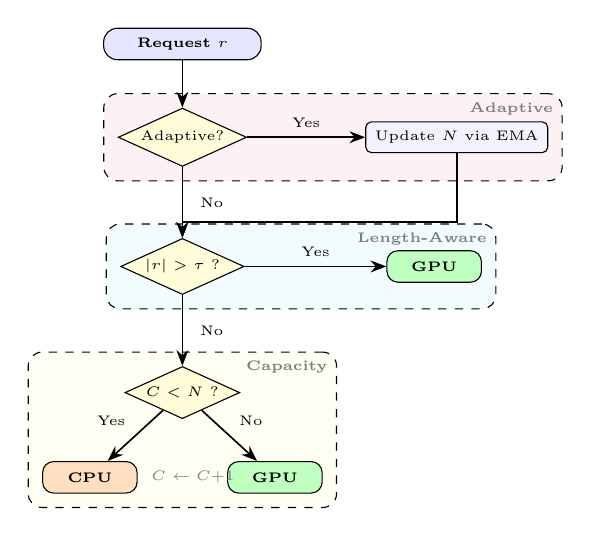
\begin{tikzpicture}[
    >=Stealth,
    node distance=0.5cm,
    start/.style={draw, rounded corners=5pt, fill=blue!10, minimum width=2cm, minimum height=0.4cm, align=center, font=\tiny\bfseries},
    decision/.style={draw, diamond, aspect=2.2, fill=yellow!15, align=center, font=\tiny, inner sep=1pt},
    result/.style={draw, rounded corners=4pt, minimum width=1.2cm, minimum height=0.4cm, align=center, font=\tiny\bfseries},
    gpu/.style={result, fill=green!25},
    cpu/.style={result, fill=orange!25},
    phase/.style={draw, dashed, rounded corners=5pt, inner sep=5pt},
    plabel/.style={font=\tiny\bfseries, text=gray},
    arrow/.style={->, semithick},
  ]
  \node[start] (entry) {Request $r$};
  \node[decision, below=0.6cm of entry] (adaptive) {Adaptive?};
  \node[draw, fill=blue!5, rounded corners=2pt, right=1.5cm of adaptive, minimum width=2cm, minimum height=0.35cm, align=center, font=\tiny] (ema) {Update $N$ via EMA};
  \node[decision, below=0.9cm of adaptive] (length) {$|r| > \tau$ ?};
  \node[decision, below=0.9cm of length] (capacity) {$C < N$ ?};
  \node[gpu, right=1.8cm of length] (gpu1) {GPU};
  \node[cpu, below left=0.7cm and 0.2cm of capacity] (cpu1) {CPU};
  \node[gpu, below right=0.7cm and 0.2cm of capacity] (gpu2) {GPU};
  \draw[arrow] (entry) -- (adaptive);
  \draw[arrow] (adaptive) -- node[above, font=\tiny] {Yes} (ema);
  \draw[arrow] (ema.south) |- ([yshift=0.2cm]length.north) -- (length.north);
  \draw[arrow] (adaptive) -- node[right, font=\tiny, xshift=0.1cm] {No} (length);
  \draw[arrow] (length) -- node[above, font=\tiny] {Yes} (gpu1);
  \draw[arrow] (length) -- node[right, font=\tiny, xshift=0.1cm] {No} (capacity);
  \draw[arrow] (capacity) -- node[above left, font=\tiny] {Yes} (cpu1);
  \draw[arrow] (capacity) -- node[above right, font=\tiny] {No} (gpu2);
  \begin{scope}[on background layer]
    \node[phase, fill=purple!5, fit=(adaptive)(ema), label={[plabel, anchor=north east]north east:Adaptive}] {};
    \node[phase, fill=cyan!5, fit=(length)(gpu1), label={[plabel, anchor=north east]north east:Length-Aware}] {};
    \node[phase, fill=yellow!5, fit=(capacity)(cpu1)(gpu2), label={[plabel, anchor=north east]north east:Capacity}] {};
  \end{scope}
  \node[font=\tiny\itshape, text=gray, anchor=west] at ([xshift=0.05cm]cpu1.east) {$C \gets C{+}1$};
\end{tikzpicture}
\caption{Routing decision flow. The three strategies are \emph{mutually exclusive} (selected via \texttt{--hybrid-routing-strategy}): \emph{capacity} uses only the bottom check ($C < N$), skipping both the adaptive and length-threshold stages; \emph{length-aware} adds the prompt-length threshold $\tau$; \emph{throughput-adaptive} adds EMA-based $N$ adjustment atop length-aware logic.}
\label{fig:routing}
\end{figure}

\subsection{Automatic CPU Configuration}
\label{sec:autoconfig}

A key barrier to heterogeneous deployment is configuration complexity.
Correctly running CPU inference requires answering multiple hardware-specific questions: How many threads should be allocated? Which NUMA node should host the inference process? How much memory can be reserved for KV cache without starving the OS or model weights? Which ISA extensions (AVX-512, VNNI, AMX) are available, and how should the math libraries be configured to exploit them?
Answering these questions manually requires deep knowledge of the target hardware's topology, and misconfiguration can severely degrade performance---e.g., binding threads to the wrong NUMA node incurs 30--40\% remote memory access penalties~\cite{lameter2013numa}, while enabling hyperthreading on memory-bound workloads causes resource contention with no throughput benefit~\cite{eyerman2010smt}.
Our system eliminates this burden through automatic hardware detection, implementing a \emph{zero-configuration} philosophy where all parameters default to zero (auto).

\begin{table}[t]
\centering
\caption{Automatic CPU parameter derivation. All parameters default to zero (auto), triggering hardware-aware inference rules.}
\label{tab:autoconfig}
\footnotesize
\begin{tabular}{@{}lll@{}}
\toprule
\textbf{Parameter} & \textbf{Auto Rule} & \textbf{Rationale} \\
\midrule
\texttt{cpu\_threads} & NUMA node phys.\ cores & Avoid HT contention \\
\texttt{max\_seqs} & max(4, $\lfloor$cores / 4$\rfloor$) & 4 threads/sequence \\
\texttt{kv\_cache\_gb} & clamp(eff\_mem $\times$ 0.4, 32, 512) & Reserve for OS/weights \\
\texttt{batch\_tokens} & max\_seqs $\times$ 256 & Typical decode length \\
\bottomrule
\end{tabular}
\end{table}

Table~\ref{tab:autoconfig} summarizes the derivation rules.
We elaborate on the rationale behind each:

\textbf{Thread count.}
When NUMA binding is active (default), the system uses only the physical cores of a single NUMA node; when NUMA is disabled or the NUMA library is unavailable, it falls back to using all physical cores across all sockets. In both cases, hyperthreads (logical cores sharing the same execution units) are excluded.
For memory-bandwidth-bound inference workloads, Simultaneous Multithreading (SMT) provides no throughput benefit because both logical threads compete for the same memory bus and cache hierarchy~\cite{eyerman2010smt}; in practice, enabling SMT for LLM decode can \emph{reduce} throughput due to increased L2/L3 cache contention.
On a dual-socket Xeon~8480+ with 56 physical cores per socket, this yields 56 threads bound to one NUMA node.

\textbf{Maximum concurrent sequences.}
Each inference sequence requires a minimum number of threads for efficient parallelism across attention heads and FFN layers.
Empirically, 4 threads per sequence provides a good balance between per-sequence latency and aggregate throughput, yielding $\max(4, \lfloor 56/4 \rfloor) = 14$ concurrent sequences for a 56-core node. The lower bound of 4 ensures a minimum level of CPU parallelism even on systems with few cores.

\textbf{KV cache allocation.}
The 40\% rule reserves sufficient memory for the operating system, model weights (which can exceed 100\,GB for 70B-parameter models), PyTorch runtime buffers, and a safety margin.
When NUMA binding is active, \texttt{eff\_mem} refers to the memory of the bound NUMA node (e.g., ${\sim}1$\,TB on a 2\,TB dual-socket server), not total system memory.
On such a node, the unclamped value is $0.4 \times 1{,}024 = 410$\,GB, within the clamp range; this suffices to hold hundreds of concurrent sequences with multi-thousand-token context lengths.
When NUMA is disabled, total system memory is used (e.g., $0.4 \times 2{,}048 = 819$\,GB, capped at the 512\,GB upper bound).

\textbf{Topology detection.}
The detection pipeline traverses the hardware topology hierarchy following the conceptual model of the hwloc framework~\cite{broquedis2010hwloc}, as illustrated in Figure~\ref{fig:hwloc}.
Rather than linking against hwloc directly, the system reads equivalent information from OS interfaces (\texttt{/proc/cpuinfo}, \texttt{lscpu}, \texttt{libnuma}) at each level:

\begin{figure*}[t]
\centering
\resizebox{0.85\textwidth}{!}{%
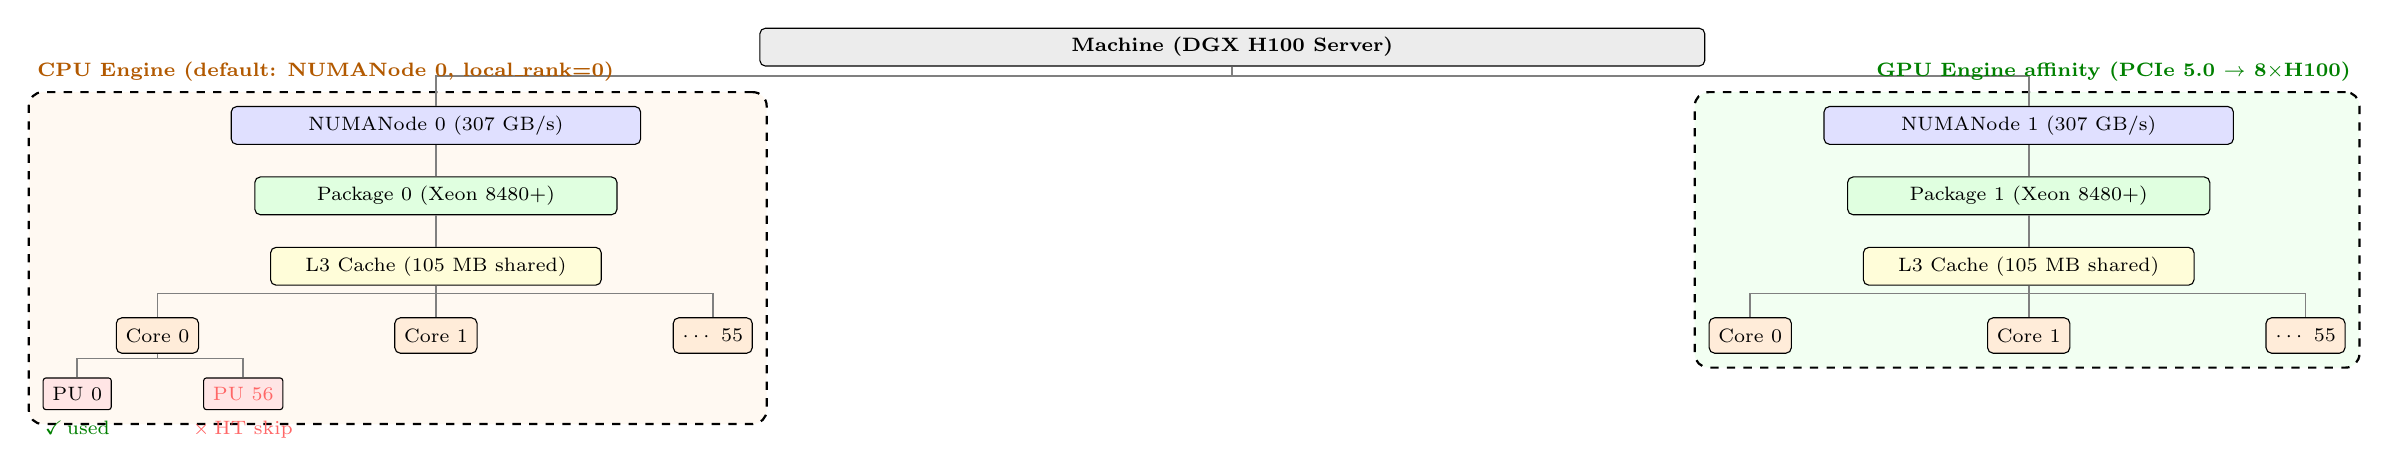
\begin{tikzpicture}[
    >=Stealth,
    node distance=0.35cm,
    lv/.style={font=\scriptsize, draw, rounded corners=2pt, minimum height=0.45cm, align=center},
    machine/.style={lv, fill=gray!15, minimum width=12cm, font=\scriptsize\bfseries},
    numa/.style={lv, fill=blue!12, minimum width=5.2cm},
    pkg/.style={lv, fill=green!12, minimum width=4.6cm},
    l3/.style={lv, fill=yellow!15, minimum width=4.2cm},
    core/.style={lv, fill=orange!15, minimum width=1.0cm},
    pu/.style={draw, fill=red!10, rounded corners=1pt, minimum width=0.6cm, minimum height=0.3cm, font=\scriptsize, align=center},
    engine/.style={draw, thick, dashed, rounded corners=5pt, inner sep=5pt},
    elabel/.style={font=\scriptsize\bfseries},
    arrow/.style={-, semithick, gray},
  ]
  \node[machine] (m) {Machine (DGX H100 Server)};
  \node[numa, below left=0.5cm and 1.5cm of m] (n0) {NUMANode 0 (307 GB/s)};
  \node[numa, below right=0.5cm and 1.5cm of m] (n1) {NUMANode 1 (307 GB/s)};
  \draw[arrow] (m.south) -- ++(0,-0.12) -| (n0.north);
  \draw[arrow] (m.south) -- ++(0,-0.12) -| (n1.north);
  \node[pkg, below=0.4cm of n0] (p0) {Package 0 (Xeon 8480+)};
  \node[pkg, below=0.4cm of n1] (p1) {Package 1 (Xeon 8480+)};
  \draw[arrow] (n0) -- (p0); \draw[arrow] (n1) -- (p1);
  \node[l3, below=0.4cm of p0] (lc0) {L3 Cache (105 MB shared)};
  \node[l3, below=0.4cm of p1] (lc1) {L3 Cache (105 MB shared)};
  \draw[arrow] (p0) -- (lc0); \draw[arrow] (p1) -- (lc1);
  % Cores socket 0
  \node[core, below left=0.4cm and 0.9cm of lc0] (ca) {Core 0};
  \node[core, below=0.4cm of lc0] (cb) {Core 1};
  \node[core, below right=0.4cm and 0.9cm of lc0] (cc) {$\cdots$ 55};
  \draw[arrow] (lc0.south) -- ++(0,-0.1) -| (ca.north);
  \draw[arrow] (lc0) -- (cb);
  \draw[arrow] (lc0.south) -- ++(0,-0.1) -| (cc.north);
  % PUs
  \node[pu, below left=0.3cm and 0.05cm of ca] (pa0) {PU 0};
  \node[pu, below right=0.3cm and 0.05cm of ca] (pa1) {\color{red!60}PU 56};
  \draw[arrow] (ca.south) -- ++(0,-0.06) -| (pa0.north);
  \draw[arrow] (ca.south) -- ++(0,-0.06) -| (pa1.north);
  \node[font=\scriptsize, color=green!50!black, below=0.02cm of pa0] {\checkmark\,used};
  \node[font=\scriptsize, color=red!60, below=0.02cm of pa1] {\texttimes\,HT skip};
  % Cores socket 1
  \node[core, below left=0.4cm and 0.9cm of lc1] (cd) {Core 0};
  \node[core, below=0.4cm of lc1] (ce) {Core 1};
  \node[core, below right=0.4cm and 0.9cm of lc1] (cf) {$\cdots$ 55};
  \draw[arrow] (lc1.south) -- ++(0,-0.1) -| (cd.north);
  \draw[arrow] (lc1) -- (ce);
  \draw[arrow] (lc1.south) -- ++(0,-0.1) -| (cf.north);
  % Engine zones
  \begin{scope}[on background layer]
    \node[engine, fill=orange!5, fit=(n0)(p0)(lc0)(ca)(cb)(cc)(pa0)(pa1)] (gz) {};
    \node[engine, fill=green!5, fit=(n1)(p1)(lc1)(cd)(ce)(cf)] (cz) {};
  \end{scope}
  \node[elabel, color=orange!70!black, anchor=south west] at (gz.north west) {CPU Engine (default: NUMANode 0, local\_rank=0)};
  \node[elabel, color=green!50!black, anchor=south east] at (cz.north east) {GPU Engine affinity (PCIe 5.0 $\to$ 8$\times$H100)};
\end{tikzpicture}%
}
\caption{Hardware topology hierarchy (hwloc model) for a dual-socket Xeon 8480+ server. By default, the CPU engine is assigned to NUMANode~0 (matching \texttt{local\_rank=0}); this can be overridden via \texttt{-{}-hybrid-numa-node} to use NUMANode~1 for PCIe contention avoidance. Only physical cores (PU~0--55) are used; hyperthreads (PU~56--111, marked \texttimes) are excluded to avoid SMT contention on memory-bound workloads.}
\label{fig:hwloc}
\end{figure*}
\begin{itemize}
\item \texttt{NUMANode}: Determines thread count and memory binding. On NUMA architectures, accessing memory attached to a remote socket incurs 30--40\% higher latency than local access~\cite{lameter2013numa}; binding threads and memory to the same NUMA node eliminates this penalty.
\item \texttt{Package}: Identifies the physical CPU socket. By default, the CPU engine uses NUMANode~0 (matching \texttt{local\_rank=0}); operators can override this via \texttt{-{}-hybrid-numa-node} to select a different socket, e.g., to minimize PCIe contention with the GPU pool.
\item \texttt{Core} vs.\ \texttt{PU}: Distinguishes physical cores from SMT threads. The system counts only physical cores to set \texttt{OMP\_NUM\_THREADS}, avoiding the SMT contention described above.
\item ISA capabilities (AVX-512, VNNI, AMX) are detected from \texttt{/proc/cpuinfo} to select the optimal compute kernel for each operation.
\end{itemize}

\textbf{Intel-specific optimizations.}
Based on the detected feature set, the system configures: OpenMP thread affinity (\texttt{KMP\_AFFINITY=granularity=fine,compact,1,0}) to pin threads to physical cores; \texttt{KMP\_BLOCKTIME=1} to reduce idle spinning power; oneDNN ISA selection (\texttt{ONEDNN\_MAX\_CPU\_ISA=AVX512\_CORE\_AMX} when AMX is available, falling back to \texttt{AVX512\_CORE\_VNNI} for non-AMX AVX-512 systems) to enable the best available matrix acceleration; and IPEX (Intel Extension for PyTorch) integration for optimized attention kernels.

\textbf{Graceful fallback.}
All detection is performed once at startup with a layered fallback chain: if IPEX is unavailable, the system uses PyTorch's native CPU backend; if NUMA libraries are missing, it falls back to standard memory allocation; if AMX is not supported, it falls back to AVX-512; and if AVX-512 is unavailable, it uses AVX2.
This ensures that the system operates correctly on any x86\_64 hardware---from a developer laptop to a production server---with zero manual configuration, while automatically exploiting the most advanced features available on each platform.

% ============================================================================
\section{Implementation}
\label{sec:impl}

\textbf{Process Lifecycle.}
The GPU and CPU engine processes are launched via Python \texttt{multiprocessing} using the framework's dynamic method selection (\texttt{get\_mp\_context()}), which defaults to ``fork'' but automatically switches to ``spawn'' when CUDA compatibility requires it; operators can override this via the \texttt{VLLM\_WORKER\_MULTIPROC\_METHOD} environment variable.
Communication uses ZMQ IPC sockets: a ROUTER socket for identity-based request dispatch and a PULL socket for collecting completions from both engines.
The CPU engine's configuration is derived from the GPU configuration via deep copy with targeted overrides: device type set to CPU, tensor parallelism disabled, KV cache redirected to DRAM, and CUDA visibility masked.

\textbf{AVX-512 Kernels.}
We implement up to five specialized C++ kernels compiled as a separate \texttt{\_C\_cpu\_ops} extension alongside the CUDA extension (all require AVX-512F; kernels (1) and (2) additionally require VNNI support and GCC ${\geq}$ 12.3):
(1)~a VNNI INT8 GEMM with 6$\times$16 micro-kernel exploiting \texttt{VPDPBUSD} (dot-product of unsigned/signed bytes with 32-bit accumulation);
(2)~Q8\_0 quantization compatible with llama.cpp format;
(3)~BF16/FP32 decode GEMV with software prefetch;
(4)~a batched attention kernel (BF16 path) that groups up to 16 sequences per batch for cache locality; within each sequence, AVX-512's 16-wide SIMD lanes are applied to head-dimension vector operations (sequences are iterated sequentially within the batch), with KV cache L2 prefetching via \texttt{\_MM\_HINT\_T1} (the FP32 path uses a simpler per-sequence implementation without batch-16 grouping but retains the same KV cache L2 prefetch pattern);
and (5)~NUMA-aware memory operations including non-temporal memcpy and node-local allocation.
ISA availability is detected at two stages: at \emph{build time}, CMake reads \texttt{/proc/cpuinfo} to decide which kernels to compile (e.g., VNNI kernels require both hardware support and GCC $\geq$ 12.3); at \emph{runtime}, a Python-side detector re-reads \texttt{/proc/cpuinfo} to set environment variables (e.g., \texttt{ONEDNN\_MAX\_CPU\_ISA}) matching the host's actual capabilities.

% ============================================================================
\section{Preliminary Analysis and Evaluation Plan}
\label{sec:eval}

This paper focuses on system design and theoretical analysis; full experimental evaluation on production hardware (8$\times$H100 + dual Xeon 8480+) is underway and will be reported in a forthcoming extended version.
We present roofline-based throughput predictions as a preliminary analysis and describe the planned experimental methodology for completeness.

\subsection{Throughput Predictions}

Table~\ref{tab:predictions} presents theoretical throughput predictions derived from the roofline model (Equation~\ref{eq:roofline}).
These are \emph{upper bounds} on single-request decode throughput that do not account for KV cache overhead, continuous batching effects, or hardware contention (see the extended model in Corollary~\ref{cor:roofline}).
The CPU contribution is most significant for smaller models where the weight-to-bandwidth ratio is favorable.

\begin{table}[t]
\centering
\caption{Predicted decode throughput (roofline upper bounds). CPU tok/s: single-request decode via Equation~\ref{eq:roofline} ($B_\text{CPU}/(P \times b)$), excluding KV cache overhead and prefill. GPU tok/s: system-level ranges from published vLLM benchmarks~\cite{kwon2023vllm} under TP=8 with continuous batching (batch size 16--64, mixed prompt lengths). \textbf{Caution:} GPU figures reflect batched system throughput while CPU figures are single-request upper bounds; actual hybrid gain will be lower once CPU continuous batching and prefill overhead are accounted for.}
\label{tab:predictions}
\footnotesize
\begin{tabular}{@{}lrrrr@{}}
\toprule
\textbf{Model} & \textbf{Quant.} & \textbf{CPU tok/s\textsuperscript{a}} & \textbf{GPU tok/s\textsuperscript{b}} & \textbf{Gain\textsuperscript{c}} \\
\midrule
LLaMA-3 70B & Q8\_0 & 4.4 & 120--200 & 2--4\% \\
LLaMA-3 8B & Q8\_0 & 38.4 & 300--500 & 8--13\% \\
Qwen-2.5 32B & Q8\_0 & 9.6 & 180--300 & 3--5\% \\
\bottomrule
\multicolumn{5}{@{}l@{}}{\scriptsize \textsuperscript{a}Single-request roofline upper bound. \textsuperscript{b}Batched system throughput.} \\
\multicolumn{5}{@{}l@{}}{\scriptsize \textsuperscript{c}Optimistic; actual gains require empirical validation.}
\end{tabular}
\end{table}

Figure~\ref{fig:throughput} visualizes these predictions, highlighting that the CPU contribution scales inversely with model size---smaller models yield proportionally larger gains because each decode step transfers fewer bytes per token.

\begin{figure}[t]
\centering
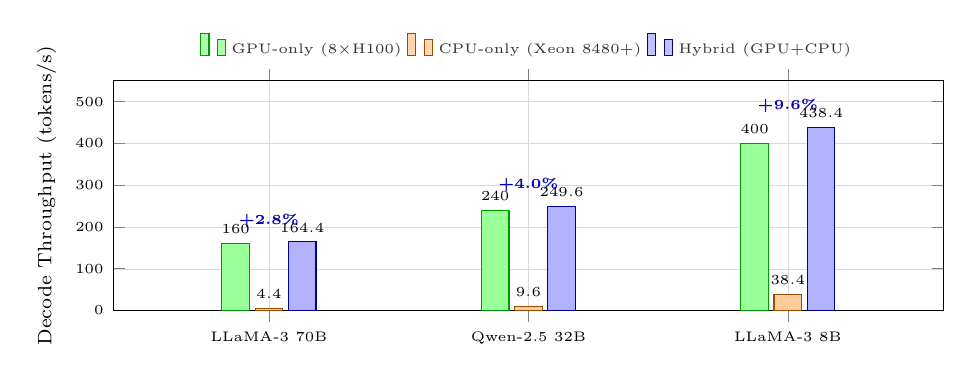
\begin{tikzpicture}
\begin{axis}[
    width=\columnwidth,
    height=4.5cm,
    ybar=2pt,
    bar width=10pt,
    ylabel={Decode Throughput (tokens/s)},
    ylabel style={font=\scriptsize},
    symbolic x coords={LLaMA-3 70B, Qwen-2.5 32B, LLaMA-3 8B},
    xtick=data,
    xticklabel style={font=\tiny, align=center},
    yticklabel style={font=\tiny},
    ymin=0, ymax=550,
    ytick={0, 100, 200, 300, 400, 500},
    legend style={at={(0.5,1.05)}, anchor=south, legend columns=3, font=\tiny, draw=none, fill=white, fill opacity=0.8},
    nodes near coords,
    every node near coord/.append style={font=\tiny, anchor=south},
    grid=major,
    grid style={line width=0.1pt, draw=gray!30},
    enlarge x limits=0.3,
  ]
  \addplot[fill=green!40, draw=green!60!black] coordinates {
    (LLaMA-3 70B, 160) (Qwen-2.5 32B, 240) (LLaMA-3 8B, 400) };
  \addplot[fill=orange!40, draw=orange!60!black] coordinates {
    (LLaMA-3 70B, 4.4) (Qwen-2.5 32B, 9.6) (LLaMA-3 8B, 38.4) };
  \addplot[fill=blue!30, draw=blue!60!black] coordinates {
    (LLaMA-3 70B, 164.4) (Qwen-2.5 32B, 249.6) (LLaMA-3 8B, 438.4) };
  \legend{GPU-only (8$\times$H100), CPU-only (Xeon 8480+), Hybrid (GPU+CPU)}
  % Gain annotations positioned relative to the Hybrid bars using axis coordinates
  \node[font=\tiny\bfseries, color=blue!70!black, anchor=south] at (axis cs:LLaMA-3 70B, 175) {+2.8\%};
  \node[font=\tiny\bfseries, color=blue!70!black, anchor=south] at (axis cs:Qwen-2.5 32B, 260) {+4.0\%};
  \node[font=\tiny\bfseries, color=blue!70!black, anchor=south] at (axis cs:LLaMA-3 8B, 450) {+9.6\%};
\end{axis}
\end{tikzpicture}
\caption{Predicted decode throughput comparison. The CPU contribution is most significant for smaller models: LLaMA-3 8B gains 9.6\% additional throughput from the CPU engine, equivalent to nearly one additional H100-equivalent stream under TP=8.}
\label{fig:throughput}
\end{figure}

\subsection{Experimental Setup}

\begin{table}[t]
\centering
\caption{Hardware and software configuration for evaluation.}
\label{tab:setup}
\footnotesize
\begin{tabular}{@{}ll@{}}
\toprule
\textbf{Component} & \textbf{Specification} \\
\midrule
GPU & 8$\times$ NVIDIA H100 80GB SXM5 \\
CPU & 2$\times$ Intel Xeon Platinum 8480+ (56C/112T) \\
Memory & 2\,TB DDR5-4800 (8 ch/socket, 307\,GB/s) \\
Interconnect & NVLink 4.0 (GPU), PCIe 5.0 (CPU-GPU) \\
\midrule
Framework & vLLM v0.7+ (modified) \\
CPU Backend & PyTorch + IPEX 2.4, llama.cpp Q8\_0 \\
OS & Ubuntu 22.04, Linux 6.5+ \\
\midrule
Models & LLaMA-3 70B (TP=8), LLaMA-3 8B \\
Workloads & ShareGPT traces, synthetic uniform \\
Metrics & Throughput, TTFT, TPOT, p99 latency, power \\
\bottomrule
\end{tabular}
\end{table}

\subsection{Planned Experiments}

We design six experiments to validate the theoretical model and characterize system behavior:

\textbf{Exp~1: End-to-end throughput.}
Compare GPU-only vLLM against hybrid mode under increasing request rates using ShareGPT traces.
We expect the hybrid system to match or exceed GPU-only throughput at all load levels, with the largest gains at high load when GPU queues build up.

\textbf{Exp~2: GPU latency impact.}
Measure p50/p95/p99 latency distributions for GPU-processed requests in both configurations.
Corollary~\ref{cor:latency} predicts no statistically significant difference, which we verify with a two-sample Kolmogorov-Smirnov test.

\textbf{Exp~3: Routing strategy comparison.}
Evaluate the three router strategies (capacity, length-aware, throughput-adaptive) across varying workload characteristics.
We hypothesize that throughput-adaptive routing performs best under bursty workloads, while capacity routing suffices for steady-state loads.

\textbf{Exp~4: Ablation study.}
Isolate the contributions of NUMA binding, IPEX optimization, and automatic configuration by selectively disabling each component and measuring the impact on CPU engine throughput.

\textbf{Exp~5: Model size scalability.}
Test with models ranging from 8B to 70B parameters to validate the roofline prediction that smaller models yield proportionally larger CPU contributions.

\textbf{Exp~6: Energy efficiency.}
Measure system power consumption using Intel RAPL (Running Average Power Limit) counters during GPU-only and hybrid operation.
We compute the performance-per-watt ratio (Equation~\ref{eq:energy}) and validate that $\eta > 1$, confirming that the marginal power increase from CPU activation is outweighed by the throughput gain.

% ============================================================================
\section{Discussion}
\label{sec:discussion}

\subsection{Energy and TCO Implications}

Our approach directly addresses the energy-proportionality gap identified by Barroso and H\"{o}lzle~\cite{barroso2007energy}.
By activating idle CPU resources for productive work, we convert the CPU subsystem from a passive power consumer to an active inference contributor.
The marginal energy cost is small: the CPU subsystem idles at ${\sim}175$\,W (both sockets combined, ${\sim}25\%$ of TDP); activating one socket for inference raises total CPU power to an estimated ${\sim}350$\,W (one socket at TDP, one idle), adding only ${\sim}175$\,W to a system already drawing over 10\,kW.
This represents a 1.7\% power increase for a projected 2--13\% throughput gain, yielding a net improvement in performance-per-watt.
These figures are \emph{projections} based on TDP specifications and the roofline throughput model; actual power draw may be lower than TDP for memory-bound workloads (typically 60--70\% of TDP), and DRAM power consumption increases under active access patterns.
Actual throughput gains may also differ due to thermal throttling, memory contention, and workload variability.
Empirical validation using Intel RAPL power counters under production workloads is planned (Section~\ref{sec:eval}, Exp~6).

From a TCO perspective, the approach requires zero additional capital expenditure---the CPU hardware is already present in every GPU server.
For a 100-node cluster, even a conservative 3\% throughput improvement delivers the equivalent capacity of three additional GPU servers, valued at approximately \$900K, while the incremental annual power cost is only \$18.4K (175\,W $\times$ 100 nodes $\times$ 8{,}760\,h $\times$ \$0.12/kWh).

\subsection{Comparison with Independent Instances}

A natural baseline is deploying two separate vLLM instances (one GPU, one CPU-only) behind an external load balancer (e.g., NGINX, Envoy).
Our unified architecture offers three advantages over this approach:
(1)~\emph{Shared request context}: the CapacityAwareRouter has direct access to CPU in-flight counts, enabling work-conserving dispatch that an external load balancer (limited to round-robin or least-connections) cannot replicate;
(2)~\emph{Automatic configuration}: the CPU engine inherits the GPU engine's model, tokenizer, and sampling parameters via config deep-copy, eliminating manual configuration synchronization;
(3)~\emph{Single API endpoint}: clients see one serving instance with consistent request IDs, simplifying monitoring and debugging.
The throughput contribution is identical in both approaches (the CPU processes the same requests either way); the difference is operational complexity and routing precision.
We acknowledge that the independent-instance approach has lower implementation complexity and may be preferable in environments where existing load-balancing infrastructure is mature.
Empirical comparison is planned as part of Exp~1.

\subsection{Extensibility}

The dual-process architecture provides a foundation for additional heterogeneous capabilities.
The CPU process can naturally serve as a target for MoE expert offloading~\cite{rajbhandari2022deepspeedmoe}, CPU-based speculative decoding (draft model on CPU, verification on GPU)~\cite{leviathan2023speculative, dovetail2024}, and can be extended to disaggregated serving topologies where CPU nodes handle overflow decode~\cite{zhong2024distserve}.

\subsection{Limitations}

Our approach has several limitations.
First, CPU throughput is inherently bounded by memory bandwidth, limiting gains for very large models (1--4\% for 70B).
Second, the CPU engine requires a \textbf{separate copy of model weights} in system memory (e.g., ${\sim}70$\,GB for a 70B Q8\_0 model), reducing the DRAM available for KV cache by that amount.
On a 1\,TB NUMA node, this overhead reduces the auto-configured KV cache from ${\sim}410$\,GB to ${\sim}340$\,GB (a 17\% reduction).
We note that this affects only the \emph{CPU} engine's KV cache capacity; the GPU engine's KV cache resides in HBM and is unaffected.
Since the CPU engine runs with a small number of concurrent sequences ($N \approx 14$ for 56 cores), this reduced KV cache is still sufficient for hundreds of concurrent sequences with multi-thousand-token contexts---the binding constraint is $N$, not KV cache size.
For very large models (e.g., 405B) that consume a substantial fraction of DRAM, the memory overhead may render CPU inference infeasible, and the system should gracefully fall back to GPU-only mode.
Additionally, model loading occurs independently in both processes, approximately doubling startup time compared to GPU-only mode.

Third, \textbf{CPU prefill latency} is substantially higher than GPU.
Even for short prompts (${\leq}512$ tokens), CPU prefill time may be $10\text{--}50{\times}$ slower than GPU due to the compute-intensive self-attention ($O(n^2)$).
This means requests routed to CPU will experience significantly higher Time-To-First-Token (TTFT), creating \emph{latency inconsistency} at the API level: users submitting identical prompts may observe widely different response times depending on routing.
This complicates Service Level Objective (SLO) definitions that bound p99 TTFT.
The length-aware routing strategy mitigates this by sending only short prompts to CPU, and for decode-heavy workloads (where TTFT is amortized over many output tokens), the impact on overall latency is reduced.
Quantifying this TTFT trade-off and its SLO implications empirically is a priority for future evaluation.

Fourth, \textbf{numerical consistency}: both engines run the same model at the same precision (BF16 or the quantization format specified by the user), so outputs are bitwise-compatible in expectation.
However, differences in floating-point reduction order between CPU and GPU implementations may produce minor numerical variations in edge cases.
For autoregressive generation, where each token depends on the previous context, these differences do not accumulate across requests because the CPU and GPU engines serve \emph{independent} requests, not different tokens of the same sequence.

Fifth, the additive throughput model assumes no hardware-level resource contention (Claim~1, condition~ii).
While NUMA binding provides natural memory bandwidth isolation on dual-socket systems, single-socket configurations may experience DDR5 contention when both the CPU engine and GPU DMA share the same memory controller.
Empirical measurement of this contention effect remains future work.

Sixth, our roofline analysis models \textbf{single-request decode throughput}; the interaction with continuous batching on the CPU engine---where multiple sequences share the memory bus and weight-loading cost is amortized---requires empirical characterization.
CPU continuous-batching throughput may differ from the single-request roofline prediction in either direction: weight amortization could improve throughput, while increased cache pressure from multiple KV caches could reduce it.

Finally, as CPU generations advance, the absolute CPU contribution grows: Granite Rapids (128 cores, 845\,GB/s) would yield $845/3{,}350 = 25.2\%$ vs.\ a single H100, and $845/(3{,}350/8) = 202\%$ of one GPU-equivalent stream under TP=8.
However, GPU bandwidth also advances: NVIDIA Blackwell B200 offers 8\,TB/s HBM3e, yielding a ratio of $845/8{,}000 = 10.6\%$---similar to today's 9.2\%.
Thus the CPU-to-GPU bandwidth ratio may remain roughly constant across generations, and the architecture's value proposition depends more on the marginal cost of CPU activation than on closing the bandwidth gap.

% ============================================================================
\section{Conclusion}
\label{sec:conclusion}

We presented the design and analysis of a dual-process parallel-batch architecture that engages both the CPU and GPU in inference computation, converting idle CPU cycles in GPU servers into productive LLM serving capacity.
By running CPU and GPU inference engines as independent OS processes, the architecture targets additive throughput ($T_\text{hybrid} = T_\text{GPU} + \alpha \cdot T_\text{CPU}$) with zero GPU performance degradation.
The self-regulating CapacityAwareRouter and zero-configuration optimization pipeline make the system practical for deployment without manual tuning.
The key claims---additive throughput and negligible hardware contention---rest on assumptions that require empirical validation; this validation on production hardware is our immediate next step.

More broadly, this work argues that \emph{idle resources are a missed opportunity, not a fixed cost}.
As server-class CPUs continue to evolve---with Granite Rapids already doubling core counts and nearly tripling memory bandwidth---the CPU's potential contribution to heterogeneous inference will only grow.
By converting idle power into useful work, our approach aims to improve server-level energy efficiency and move GPU inference infrastructure closer to the ideal of energy-proportional computing.

% ============================================================================
\section*{Acknowledgment}
During the preparation of this work, the authors used Claude (Anthropic) to assist with literature survey, manuscript drafting, and \LaTeX{} formatting across multiple sections.
All AI-generated content was critically reviewed, verified, and edited by the authors, who take full responsibility for the content of this publication.

% ============================================================================
\balance
\bibliographystyle{IEEEtran}
\bibliography{references}

\end{document}
